\section{Results: The Decomposition}
\label{sec:results}

\subsection{Accuracy and cost on four models}
\label{sec:headline}

\begin{table*}[t]
\centering
\small
\begin{tabular}{@{}lrrrr@{}}
\toprule
\tabhead{Arm} & \tabhead{Overall} & \tabhead{Hard} & \tabhead{Easy} & \tabhead{Cost} \\
\midrule
\multicolumn{5}{@{}l}{\emph{\mGLM{} (\texttt{glm-5.3-flash}, 401 tasks)}}\\
\armS{} & 22.7\% & 13.9\% & 65.2\% & \$0.76 \\
\armH{} & 26.4\% & 19.3\% & 60.9\% & \$0.85 \\
\armM{} & 31.7\% & 22.9\% & 73.9\% & \$0.96 \\
\armC{} & \textbf{57.9\%} & \textbf{55.1\%} & 71.0\% & \textbf{\$0.67} \\
\midrule
\multicolumn{5}{@{}l}{\emph{\mDS{} (\texttt{deepseek-v4-flash}, 279 tasks)}}\\
\armS{} & 33.0\% & 22.6\% & 77.4\% & \$1.79 \\
\armH{} & 31.5\% & 22.6\% & 69.8\% & \$1.52 \\
\armM{} & 52.0\% & 42.9\% & 90.6\% & \$1.69 \\
\armC{} & \textbf{61.3\%} & \textbf{56.6\%} & 81.1\% & \textbf{\$1.05} \\
\midrule
\multicolumn{5}{@{}l}{\emph{\mSON{} (Claude Sonnet~5, 401 tasks)}}\\
\armS{} & 31.9\% & 22.9\% & 75.4\% & \textbf{\$36.80} \\
\armH{} & 44.4\% & 38.0\% & 75.4\% & \$46.08 \\
\armM{} & 35.2\% & 23.8\% & 89.9\% & \$43.89 \\
\armC{} & \textbf{69.6\%} & \textbf{68.4\%} & 75.4\% & \$37.97 \\
\midrule
\multicolumn{5}{@{}l}{\emph{\mGPT{} (\texttt{gpt-5.6-sol}, 401 tasks)}}\\
\armS{} & 43.9\% & 37.0\% & 76.8\% & \$14.52 \\
\armH{} & 55.6\% & 51.2\% & 76.8\% & \$22.09 \\
\armM{} & 57.9\% & 50.3\% & 94.2\% & \textbf{\$14.42} \\
\armC{} & \textbf{78.8\%} & \textbf{77.4\%} & 85.5\% & \$21.32 \\
\bottomrule
\end{tabular}
\caption{Accuracy and cost, models in order of bare-schema capability. Hard
splits are $n{=}332$, 226, 332 and 332; easy are 69, 53, 69 and 69. \armC{}
is the most accurate arm on all four models, the cheapest on the two flash
models, and within about 3\% of the cheapest on \mSON{}. Arms are in ladder
order, so the two content-free arms are adjacent.}
\label{tab:headline}
\end{table*}

\begin{table*}[t]
\centering
\small
\setlength{\tabcolsep}{4pt}
\begin{tabular}{@{}lrrrr@{}}
\toprule
\tabhead{Comparison} & \mGLM{} & \mDS{} & \mSON{} & \mGPT{} \\
\midrule
\armS{} vs \armC{} & $3{\times}10^{-31}$ \,\, 14/\textbf{155} & $2{\times}10^{-15}$ \,\, 14/\textbf{93} & $1{\times}10^{-35}$ \,\, 11/\textbf{162} & $5{\times}10^{-32}$ \,\, 12/\textbf{152} \\
\armM{} vs \armC{} & $2{\times}10^{-17}$ \,\, 29/\textbf{134} & \textbf{0.0067} \,\, 30/\textbf{56} & $5{\times}10^{-27}$ \,\, 22/\textbf{160} & $2{\times}10^{-17}$ \,\, 12/\textbf{96} \\
\armH{} vs \armC{} & $9{\times}10^{-24}$ \,\, 23/\textbf{149} & $8{\times}10^{-17}$ \,\, 13/\textbf{96} & $2{\times}10^{-17}$ \,\, 25/\textbf{126} & $2{\times}10^{-17}$ \,\, 18/\textbf{111} \\
\armS{} vs \armM{} & $7{\times}10^{-6}$ \,\, 14/50 & $2{\times}10^{-12}$ \,\, 5/58 & \textbf{0.066} \,\, 15/28 & $2{\times}10^{-8}$ \,\, 22/78 \\
\armM{} vs \armH{} & 0.033 \,\, 55/34 & $4{\times}10^{-13}$ \,\, 63/6 & $1{\times}10^{-4}$ \,\, 27/\textbf{64} & 0.44 \,\, 58/49 \\
\armS{} vs \armH{} & \textbf{0.058} \,\, 20/35 & \textbf{0.61} \,\, 19/15 & $\mathbf{9{\times}10^{-9}}$ \,\, 14/\textbf{64} & $\mathbf{4{\times}10^{-7}}$ \,\, 20/\textbf{67} \\
\bottomrule
\end{tabular}
\caption{Every pairwise paired McNemar over all tasks: $p$-value, then
discordant pairs won by the left arm / by the right arm. The last row is the
scaffolding step of the decomposition, on which the flash and frontier
models split two and two. \mSON{}'s fourth row is its own result: the pasted
manual is not distinguishable from a bare schema.}
\label{tab:mcnemar}
\end{table*}

\armC{} wins every comparison over all tasks on all four models
(Tables~\ref{tab:headline} and~\ref{tab:mcnemar}), by 32.2, 13.7, 44.6 and
27.1 hard-task points over \armM{}. That margin is not monotone in
capability, and four points cannot support a story about why
(\appref{app:interaction}). On the two flash models \armC{} is also
the cheapest arm outright; on \mSON{} it is within about 3\% of the
cheapest; on \mGPT{} the \armM{} arm is cheaper, and
Section~\ref{sec:efficiency} says why.

Two checks tie the harness to the leaderboard. \armM{} reproduces the
published band where a comparison exists: 22.9\% hard on \mGLM{} against
the 20--26\% band for named entrants (18.8\% graded officially), and 23.8\%
on \mSON{} against the leaderboard's 19.8\% for Claude~4 Sonnet under the
same approach; on \mDS{} and \mGPT{} the same arm reaches 42.9\% and
50.3\%, above the band, which is a statement about those models. The check
is looser than it looks and in a direction that favours us, because our
grading runs 3 to 6 points high on the hard split (Section~\ref{sec:golds},
\appref{app:leniency}). The easy split is the negative check: \armC{} is not
the best arm on easy tasks on any model, and \armM{} leads on all four
(73.9\%, 90.6\%, 89.9\% and 94.2\% against 71.0\%, 81.1\%, 75.4\% and
85.5\%). The contract does nothing for questions that need no domain
knowledge, which is what it should do; an instrument that showed a contract
effect there would be measuring itself. On \mSON{} the lead is an
interaction rather than noise (62 of 69 against exactly 52 for each other
arm), and none of it is fee semantics: four of the 13 tasks involved have
their answer printed verbatim in \texttt{manual.md}, and on the rest \armC{}
returned prose the scorer cannot parse, or an ordinary near-miss.

\paragraph{On one model the manual is indistinguishable from a bare schema
on hard tasks.} \mSON{}'s \armM{} scores 79 of 332 hard tasks against
\armS{}'s 76: paired McNemar $p{=}0.72$, 17 discordant pairs one way and 14
the other. The same 24{,}177-character prompt that lifts \mGLM{} by 9 points
and \mDS{} by 20 lifts \mSON{} by less than one; the contract carrying the
same knowledge lifts it by 45.5. It is also the only model on which empty
governed tools beat the whole manual by a significant margin (38.0\%
against 23.8\%, hard split $p{=}6{\times}10^{-8}$, 15/62). One alternative is not excluded: that prompt
puts 191k input tokens per task in front of \mSON{} against \armS{}'s 91k,
and a context-load effect would produce the same null. The clause analysis
of Section~\ref{sec:clauses} cannot separate the two, since rules absent from
the SQL is what both predict.

\subsection{Content dominates scaffolding}
\label{sec:decomposition}

\begin{figure}[t]
\centering
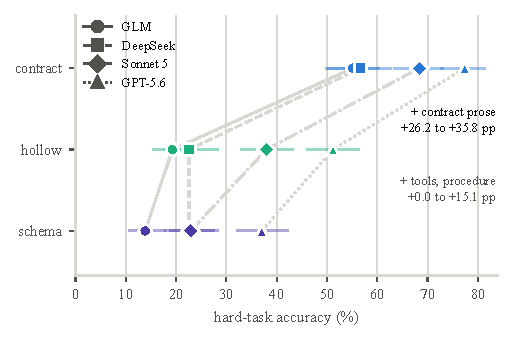
\includegraphics[width=\columnwidth]{figures/fig-ladder.pdf}
\caption{The two steps of the decomposition on hard tasks, four models in
order of bare-schema capability. Adding the nine governed tools, the
retrieval instruction, the table allow-list and the operation rules with
the prose emptied (\armS{} to \armH{}) moves accuracy by $+5.4$, $+0.0$,
$+15.1$ and $+14.2$ points; restoring the prose (\armH{} to \armC{}) moves
it by a further $+35.8$, $+34.0$, $+30.4$ and $+26.2$. Bars are Wilson
95\% intervals.}
\label{fig:ladder}
\end{figure}

On hard tasks the gain splits into a scaffolding step, \armS{} to \armH{},
and a content step, \armH{} to \armC{}: 13.9 to 19.3 to 55.1 on \mGLM{},
22.6 to 22.6 to 56.6 on \mDS{}, 22.9 to 38.0 to 68.4 on \mSON{}, and 37.0 to
51.2 to 77.4 on \mGPT{} (Figure~\ref{fig:ladder}; the same rows in
Table~\ref{tab:headline}, and the last row of Table~\ref{tab:mcnemar}).

The content step is the larger of the two on every model. The scaffolding
step depends on the model: $+5.4$ on \mGLM{} ($p{=}0.058$ over all tasks,
20/35; on the hard slice alone $p{=}0.015$), $+0.0$ on \mDS{} ($p{=}0.61$,
19/15), $+15.1$ on \mSON{} ($p{=}9{\times}10^{-9}$, 14/64) and $+14.2$ on
\mGPT{} ($p{=}4{\times}10^{-7}$, 20/67). Three of the four models favour the
scaffolding and one is flat, and the two that favour it most are from
different model families.

The claim the hollow arm was built to test survives. The sceptical reading, that
the contract helps through a narrowed table surface, an imposed procedure,
or simply by making the agent slow down, predicts that \armH{} captures most
of the gain. It does not, on any model: the content step is $6.6{\times}$
the scaffolding step on \mGLM{}, the whole of the effect on \mDS{},
$2.0{\times}$ on \mSON{} and $1.8{\times}$ on \mGPT{}. \textbf{Scaffolding is a real
but secondary effect that the content dominates everywhere.} On the two
flash models alone this step would have read as a null;
Section~\ref{sec:power} says why that would have been weak evidence.

\paragraph{Empty tools are not free.} \armH{} is the most expensive arm on
both frontier models (\$46.08 on \mSON{}, \$22.09 on \mGPT{}), makes the
most tool calls on three of the four, burns the most reasoning on \mGLM{}
and \mSON{}, and forces answers on three models where \armC{} forces none
(Table~\ref{tab:efficiency}). The transcripts show why: the agent calls
\texttt{lookup\_domain}, is told nothing is available, and searches harder.
On \mSON{} it makes that call 392 times, plus 1{,}620 calls to
\texttt{lookup\_metric} with every metric emptied; on \mGPT{}, on 401 of
401 tasks. The
models that gain most from the scaffolding are also the ones that exercise
the lookup tools hardest.

\subsection{The compiled ceiling and the derivation gap}
\label{sec:ceiling}

Every result so far compares arms to each other. None says how much of the
contract's own content an agent recovers, because nothing establishes what
recovering all of it would look like. The contract lets us establish that.
Transcribing its \texttt{sql\_expression} fields into two DuckDB views (the
fee-rule match predicate, the natural-month reconstruction, the monthly
volume and fraud-level aggregates, the fee formula, and the sum over matched
transaction--rule pairs) gives a pre-computed fee layer of the kind a
context-layer product ships. Nothing in it is authored independently of the
contract; the only work the transcription adds is composition.

Which tasks the views cover is decided from question text alone, never
from gold and never from any arm's output. DABStep's tasks are instances of
parameterised question shapes (Section~\ref{sec:dabstep}), and five of
those shapes, in eleven date and grouping variants, ask exactly what the
views compute: the total fees a merchant paid in a period, the fee rules
that applied to it, the merchants a rule applies to, the average fee for a
transaction profile, and the rules matching an account type and ACI. A
regular expression per shape matches 176 of the 401 tasks, all hard.
Instantiating the views with each task's own parameters and grading the
result with the official scorer gives the ceiling: \textbf{the compiled
contract reproduces the benchmark's gold answer on every one of the 176
tasks it covers.} This is a statement about the artifact, not about an
agent, and it has two uses. It answers the objection that \armC{} wins
because the contract is subtly wrong in a benchmark-favouring way: it
compiles to gold. And it converts accuracy into recovery against a proven
ceiling. We call the 176 the \emph{macro} bucket. Of the remaining tasks,
148 need the same semantics plus a counterfactual or an optimisation the
views do not encode (\emph{derived}), and 77 involve no fee semantics. A
layer compiled from a domain contract's declared expressions therefore
reaches 53\% of this benchmark's hard set, a bound on that kind of layer
rather than on pre-computation in general (Section~\ref{sec:prior}). On
the 176, whatever an agent fails to get is a failure to derive
(Table~\ref{tab:buckets}; \appref{app:golds} says which of the 176 share a
premise with the gold verification).

\begin{table*}[t]
\centering
\small
\setlength{\tabcolsep}{4pt}
\begin{tabular}{@{}lrrrrrrrr@{}}
\toprule
& \multicolumn{2}{c}{\mGLM{}} & \multicolumn{2}{c}{\mDS{}} & \multicolumn{2}{c}{\mSON{}} & \multicolumn{2}{c}{\mGPT{}} \\
\cmidrule(lr){2-3}\cmidrule(lr){4-5}\cmidrule(lr){6-7}\cmidrule(lr){8-9}
Hard tasks & \emph{macro} & \emph{derived} & \emph{macro} & \emph{derived} & \emph{macro} & \emph{derived} & \emph{macro} & \emph{derived} \\
\midrule
\armS{} & 2.8\% & 25.0\% & 8.5\% & 34.7\% & 6.8\% & 37.8\% & 31.8\% & 41.2\% \\
\armH{} & 10.2\% & 25.7\% & 10.2\% & 31.7\% & 36.4\% & 37.2\% & 46.6\% & 54.1\% \\
\armM{} & 14.8\% & 32.4\% & 38.1\% & 44.6\% & 8.5\% & 38.5\% & 49.4\% & 48.6\% \\
\armC{} & \textbf{60.8\%} & \textbf{45.9\%} & \textbf{62.7\%} & \textbf{46.5\%} & \textbf{73.9\%} & \textbf{60.1\%} & \textbf{94.9\%} & \textbf{56.1\%} \\
\midrule
\emph{compiled contract} & \emph{100\%} & --- & \emph{100\%} & --- & \emph{100\%} & --- & \emph{100\%} & --- \\
\bottomrule
\end{tabular}
\caption{Hard tasks split by whether the compiled contract answers the task
outright (\emph{macro}, $n{=}176$; 118 on \mDS{}'s complete-case set) or
requires reasoning on top of it (\emph{derived}, $n{=}148$; 101). The gap
between \armC{} and the compiled contract on \emph{macro} is derivation
failure on information the agent provably had.}
\label{tab:buckets}
\end{table*}

Three readings follow.

\textbf{The contract's advantage concentrates where its semantics apply
directly.} Over \armS{} it is $+58.0$, $+54.2$, $+67.1$ and $+63.1$ points on
\emph{macro} against $+20.9$, $+11.8$, $+22.3$ and $+14.9$ on \emph{derived}.
This is the domain-specificity of Section~\ref{sec:domain}, measured on a
cleaner boundary.

\textbf{The two buckets do not move together.} \armC{} scores 60.8\%, 62.7\%,
73.9\% and 94.9\% on \emph{macro}, rising with capability (with one caveat:
\mDS{} and \mSON{} are 0.3 points apart on the capability axis and 11 apart
here), against 45.9\%, 46.5\%, 60.1\% and 56.1\% on \emph{derived}, which
rises under no ordering: \mSON{} leads it while trailing \mGPT{} by 21
points on \emph{macro}.

\textbf{The derivation gap closes with capability.} Read against the
ceiling, the \emph{macro} series is a shortfall of 39.2, 37.3, 26.1 and 5.1
points below an accuracy proven reachable: the \emph{derivation gap}, the
price of making an agent derive a query the contract could have
pre-computed. Against a ceiling of 100\% the gap is arithmetically the arm's
error rate, and ``errors fall as models improve'' is not a finding. The
finding is the contrast with \emph{derived}, whose shortfall we call the
\emph{composition gap}: between the flash models and the strongest one, the same capability increment closes 87\% of the
macro-bucket gap and 19\% of the derived-bucket one, and \mSON{}'s
\emph{macro} score falls between the flash models and \mGPT{} while its
\emph{derived} score exceeds all three. We recorded the direction of this
result publicly before \mGPT{} ran, predicting a \emph{macro} score ``well
above 62.7\%, moving toward 100\%'' if capability governed it and ``near
61--63\%'' if the harness did; the observed value is 94.9\%. \mSON{}, run
last and outside the prediction, lands at 73.9\%: the direction replicated,
the size did not.

This bears on the economics of Section~\ref{sec:intro}. The derivation gap
is exactly what separates a declarative contract, which requires the agent
to derive the query, from pre-computed macros, which do not. A gap fixed
near 38 points would be a standing structural cost of the declarative
approach. A gap that falls to 5 points on the strongest model is a
\emph{transient} cost, one the trend in model capability is already paying
down, while the per-metric authoring cost of a macro layer is paid down by
nothing. What survives the strongest model is not difficulty in knowing the
domain but the counterfactual and optimisation reasoning built on top of it,
on which the four models have no clean ordering.

\subsection{The gain stays inside the contract's domain}
\label{sec:domain}

DABStep's hard set is dominated by one question family: 294 of 332 hard
tasks concern fees, and the contract encodes fee semantics. On those 294 the
contract arm scores 59.2\%, 61.2\%, 73.5\% and 83.7\% against the manual
arm's 24.5\%, 44.9\%, 24.1\% and 53.4\%. On the 38, 30, 38 and 38 hard tasks
that do not concern fees it holds no detectable advantage (9 against 4, 8
against 9, 11 against 8 and 11 against 10 correct), and on \mGPT{} the bare
schema leads the slice outright at 14, the only slice in the four runs where
it does (\appref{app:domain}). Thirty of the 38 are one family, which needs
the fee rules without naming them and scores 0 to 3 of 30 for every arm on
three of the four models. The slices are too small to be a negative result
and equally unable to support a general claim. ``Hard accuracy'' on this
benchmark is close to ``fee-question accuracy'', so the result should be
stated as: \textbf{a contract carrying a domain's semantics produces a large
gain on questions in that domain.} That is what a domain contract should do,
and it is why this benchmark cannot answer the general question.
